

\section{Comparison With Other Algorithms}
This chapter focus on the comparison of our implementation with existing other implementation in MobilityDB.  This section presents a comparison of SQUISH-E and the algorithms that are implemented in MobilityDB based on several metrics. To find out whether the SQUISH-E points at the output compete with the algorithms existing when we replicate them, we will also derive the competitiveness factor, which is essentially performance and similarity. Tests and results are retrieved through MobilityDB and processed from a custom front-end under react and grafana to obtain an analytical dashboard. Only versions that have been implemented in MobilityDB will be compared.

\subsection{Douglas-Peucker}

Douglas-Peucker is a trajectory simplification method based on offline execution, as stated in the state of the art. Thus, for it to function correctly, the entire trajectory is required.

\paragraph{Performance}
Different input settings were used to run the executions at different point sizes. In order to approximate compression ratios between 90\% and 1\%, lambda variables were selected. To highlight the algorithm's performance, the points are actually in the same location and have no actual geographical position.

\begin{table}
    \centering
    \label{tab:execution_time_douglas}
    \begin{tabular}{@{}lccccc@{}}
        \toprule
        Number of Points & \multicolumn{5}{c}{Lambda} \\
        \cmidrule{2-6}
        & 5         & 2       & 0.02        & 0.002       & 0.0002       \\
        \midrule
        100              & 00.000075 & 00.000107 & 00.000691 & 00.000581 & 00.000606 \\
        1000             & 00.00019  & 00.000194 & 00.056759 & 00.055591 & 00.056859 \\
        10000            & 00.001531 & 00.001675 & 05.721065 & 05.798434 & 05.600994 \\
        100000           & 00.017149  & 00.013302  & EOF & EOF & EOF \\
        1000000          & 00.169507 & 00.147934 & EOF & EOF & EOF \\
        \bottomrule
    \end{tabular}
    \caption{Average Execution Time for varying Number of Points and Distance values for Douglas-Peucker algorithm.}
\end{table}

The table \ref{tab:execution_time_douglas} displays the results for the number of input points and the lambda parameter provided to Douglas-Peucker.
It's amazing how fast the algorithm is for lambda=5. While the program executes in PostgreSQL, its performance is faster than that of an operation in C.  This is due to the nature of Douglas-Peucker, which avoids unnecessary simplifications and begins with the edges. We can also see that for values less than or equal to 0.02, the process is slow and even results in EOFs. 

Simplifications at a rate of less than 50\% Douglas-Peucker are quite fast. However, when the compression must be above a certain threshold, which depends on any trajectory as the parameter is an error distance rather than a compression rate, it becomes quite slow compared to its sibling SQUISH-E.  As can be seen above, SQUISH-E is the slowest with a compression ratio of 50\% and is quite consistent.


\paragraph{Similarity}
Similarity is a key metric for comparing these two algorithms with two different inputs, thus to make a comparison, consider the level of compression at the output. 


\begin{table}
	\centering
	\label{tab:douglas_vs_squish_comparison}
	\begin{tabular}{@{}lccc@{}}
		\toprule
		& \multicolumn{3}{c}{\textbf{Douglas}} \\
		\cmidrule(l){2-4}
		\textbf{SquishE} & 0.02 & 0.002 & 0.0002 \\
		\midrule
		\textbf{1x} 	& 18 	& 67 & 768 \\
		Frechet 		& -3015 & -3215 & -617.274 \\
		Hausdorff 		& -3015 	& -3215 & -617.274 \\
		DTW 			& -90073593 	& -15597514 & -5325534 \\
		Temporal 		& 1899 	& 129.712 & 1.397 \\ \midrule
		\textbf{2x} 	& 36 & 134 & 1536 \\
		Frechet 		& -28363 & -6034 & -617.274 \\
		Hausdorff 		& -28363 & -6034 & -617.274 \\
		DTW  		& -262452925 & -47034601 & -8163405 \\
		Temporal 	& 102 & 19.191 & -1.590 \\ 
		\bottomrule
	\end{tabular}
	\caption{Comparison of differences between the Douglas-Peucker and SQUISH-E (1x,2x) algorithms using Frechet, Hausdorff, and DTW distance metrics for Trajectory 1.}
\end{table}

\begin{table}
	\centering
	\label{tab:douglas_vs_squish_comparison_2}
	\begin{tabular}{@{}lccc@{}}
		\toprule
		& \multicolumn{3}{c}{\textbf{Douglas}} \\
		\cmidrule(l){2-4}
		\textbf{SquishE} & 0.02 & 0.002 & 0.0002 \\
		\midrule
		\textbf{3x} 	& 54 & 201 & 2304 \\
		Frechet 		& -34532 & -8073 & -617.274 \\
		Hausdorff 		& -34532 & -8073 & -617.274 \\
		DTW 		& -299629282 & -60327008 & -9036166 \\
		Temporal 			& -149 & -12.72 & -1.933 \\ \midrule
		\textbf{4x} 	& 72 & 268 & 3072 \\
		Frechet 		& -36615 & -10146 & -617.274 \\
		Hausdorff 		& -36615 & -10146 & -617.274 \\
		DTW 		& -325049247 & -65978902 & -9504295 \\
		Temporal 			& -278 & -22.036 & -2.315 \\
		\bottomrule
	\end{tabular}
	\caption{Comparison of differences between the Douglas-Peucker and SQUISH-E (3x,4x) algorithms using Frechet, Hausdorff, and DTW distance metrics for Trajectory 1.}
\end{table}

The tables \labelcref{tab:douglas_vs_squish_comparison,tab:douglas_vs_squish_comparison_2} compare the distances between the two algorithms. The different boxes reflect the number of points SQUISH-E generates as compared to Douglas-Peucker.
If the result is negative, SQUISH-E outperforms Douglas-Peucker. For spatial distances like Frechet and Hausdorff, we can observe that SQUISH-E with the same number of points performs better. SQUISH-E, on the other hand, has a bigger temporal area than Douglas-Peucker, indicating that SQUISH-E's gap regions are larger than Douglas-Peucker's. It competes with Douglas-Peucker at x3 for tiny percentages, but at x2 when the number of points is greater.




\subsection{MinDist}
\paragraph{Performance}
MinDist is another algorithm implemented in MobilityDB. Like SQUISH-E, MinDist operates iteratively, updating its state for each point. Its iterative structure allows it to function effectively in an online setting.

\begin{table}
    \centering
    \label{tab:execution_time_mindist}
    \begin{tabular}{@{}lccccc@{}}
        \toprule
        Number of Points & \multicolumn{5}{c}{Lambda} \\
        \cmidrule{2-6}
        & 5         & 2       & 0.02        & 0.002       & 0.0002       \\
        \midrule
        100              & 00.000021 & 00.000006 & 00.000023 & 00.000014 & 00.000016 \\
        1000             & 00.000041  & 00.000036 & 00.00012 & 00.00012 & 00.000123 \\
        10000            & 00.000291 & 00.000293 & 00.001307 & 00.00134 & 00.001449 \\
        100000           & 00.003088  & 00.003044  & 00.015219 & 00.015609 & 00.016354 \\
        1000000          & 00.034338 & 00.036202 & 00.152152 & 00.163061 & 00.178996 \\
        \bottomrule
    \end{tabular}
    \caption{Average Execution Time across varying Number of Points and Distance values for the MinDist Algorithm.}
\end{table}

In terms of performance, MinDist outperforms SQUISH-E. However, MinDist experiences a decrease in speed as the lambda variable increases.

\paragraph{Similarity}
As in the previous section, the table below shows the similarity comparison between MinDist and SQUISH-E.

\begin{table}
	\centering
	\label{tab:mindist_vs_squish_comparison}
	\begin{tabular}{@{}lccc@{}}
		\toprule
		& \multicolumn{3}{c}{\textbf{Mindist}} \\
		\cmidrule(l){2-4}
		\textbf{SquishE} & 0.02 & 0.002 & 0.0002 \\
		\midrule
		\textbf{1x} 	& 418 	& 3652 & 16919 \\
		Frechet 		& 2842.859 & 582.269 & 33.645 \\
		Hausdorff 		& 2842.859 	& 582.269 & 33.645 \\
		DTW 			& 1834655 	& 95109 & 21682 \\
		Temporal 		& 1.54 	& 0.158 & 0.091 \\ \midrule
		\textbf{2x} 	& 836 & 134 & ALL \\
		Frechet 		& 598.393 & 582.269 & -66.409 \\
		Hausdorff 		& 598.393 & 582.269 & -66.409 \\
		DTW  		& -3452102 & -463775 & -36834 \\
		Temporal 	& -3.687 & -0.563 & -0.647 \\ 
		\bottomrule
	\end{tabular}
	\caption{Comparison of differences between the MinDist and SQUISH-E (1x,2x) algorithms using Frechet, Hausdorff, and DTW distance metrics for Trajectory 1.}
\end{table}

\begin{table}
	\centering
	\label{tab:mindist_vs_squish_comparison_2}
	\begin{tabular}{@{}lccc@{}}
		\toprule
		& \multicolumn{3}{c}{\textbf{Mindist}} \\
		\cmidrule(l){2-4}
		\textbf{SquishE} & 0.02 & 0.002 & 0.0002 \\
		\midrule
		\textbf{3x} 	& 1254 & 201 & // \\
		Frechet 		& 598.393 & 582.269 &  // \\
		Hausdorff 		& 598.393 & 582.269 &  // \\
		DTW 		& -5014557 & -655462 &  // \\
		Temporal 			& -4.926 & -1.192 & // \\ \midrule
		\textbf{4x} 	& 1672 & 268 &  // \\
		Frechet 		& 598.393 & 582.269 &  // \\
		Hausdorff 		& 598.393 & 582.269 &  // \\
		DTW 		& -5960279 & -768674 &  // \\
		Temporal 			& -5.538 & -1.764 &  // \\
		\bottomrule
	\end{tabular}
	\caption{Comparison of differences between the MinDist and SQUISH-E (3x,4x) algorithms using Frechet, Hausdorff, and DTW distance metrics for Trajectory 1.}
\end{table}


The tables \labelcref{tab:mindist_vs_squish_comparison,tab:mindist_vs_squish_comparison_2} demonstrate MinDist's remarkable accuracy. SQUISH-E competes with MinDist for twice as many output points, but it is less accurate for spatial metrics like Frechet and Hausdorff. MinDist offers a remarkable balance of performance and precision. MinDist can also be used in a streaming model, but it just takes distance as input, whereas SQUISH-E in our version only takes percentage of preservation. We can also see that SQUISH-E competes with MinDist when the number of points is multiplied by two in spatiotemporal metrics like DTW and temporal. A dashboard will be installed to gain a better understanding of power and comparison, as well as observations on different sorts of trajectories.

\subsection{DashBoard}

A dashboard can help us visualize and understand our data while also providing a clear overview. The dashboard is powered by Grafana and enables for the collection and analysis of data via graphs. We can also specify that the data is pre-processed by a script in order to save analysis time and simplify the dashboard's duty.

\begin{figure}
	\centering
	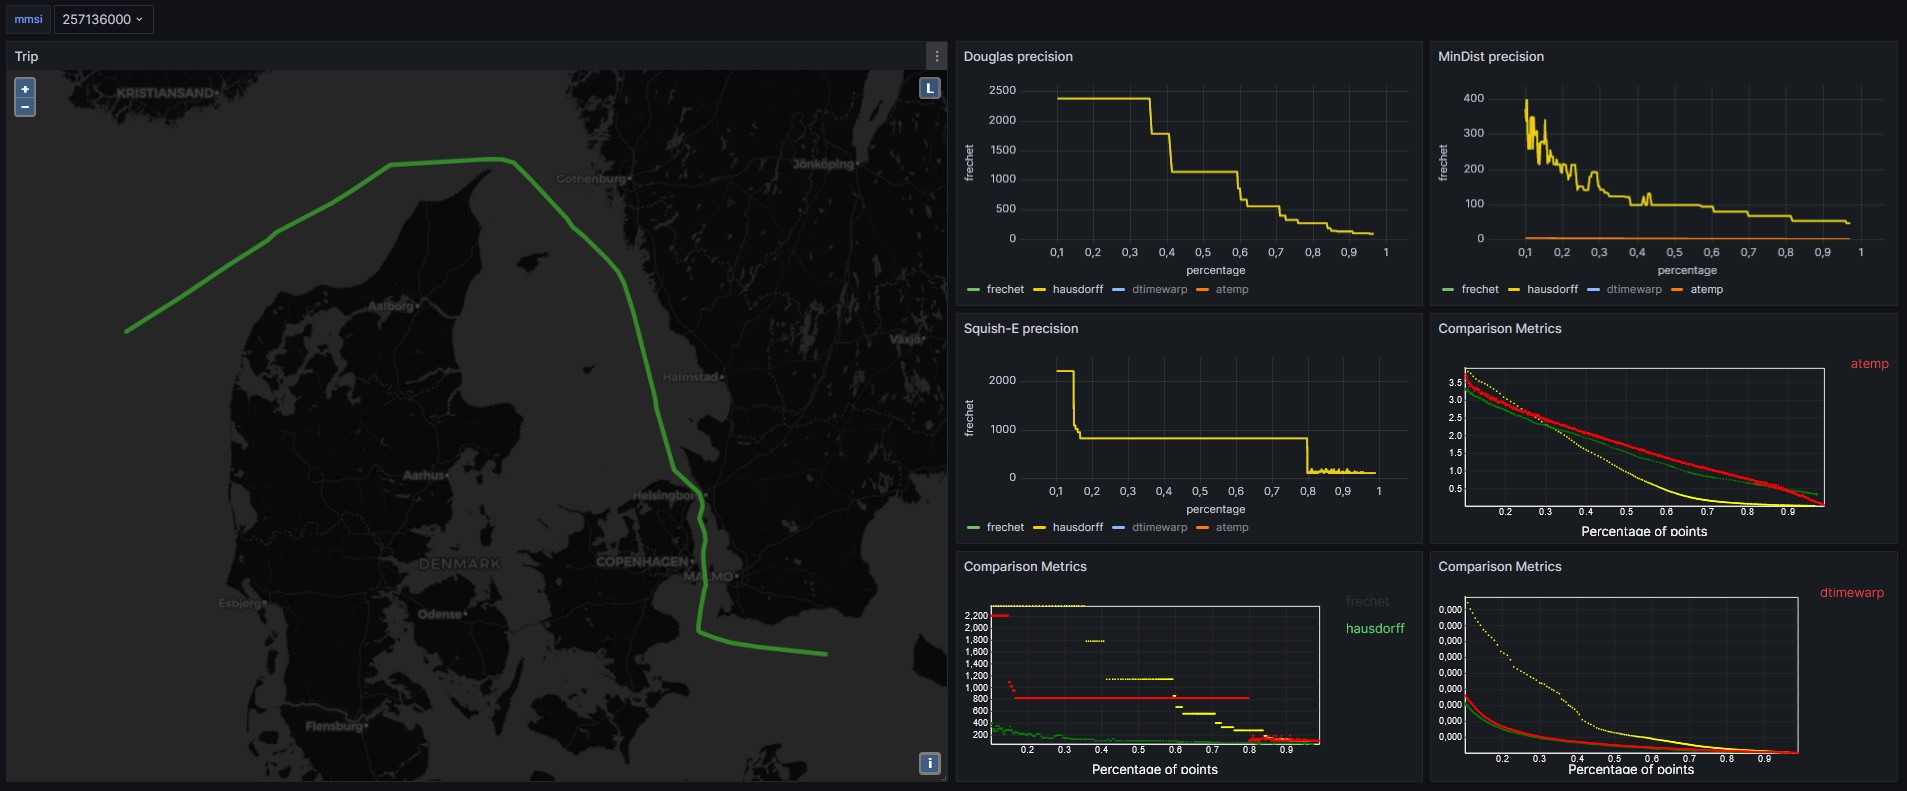
\includegraphics[width=1\linewidth]{figures/Stats/DashBoard3.jpg}
	\caption{Screenshot of the Dashboard. }
	\label{fig:dash}
\end{figure}

Figure \ref{fig:dash} shows a dashboard separated into boxes, one for each algorithm and three for each comparison.  We may compare the precision (Frechet, Hausdorff, and DTW) distances of the various compression techniques for each trajectory. This tool is powerful enough to collect analysis data on simplifications.  


\begin{figure}
	\centering
	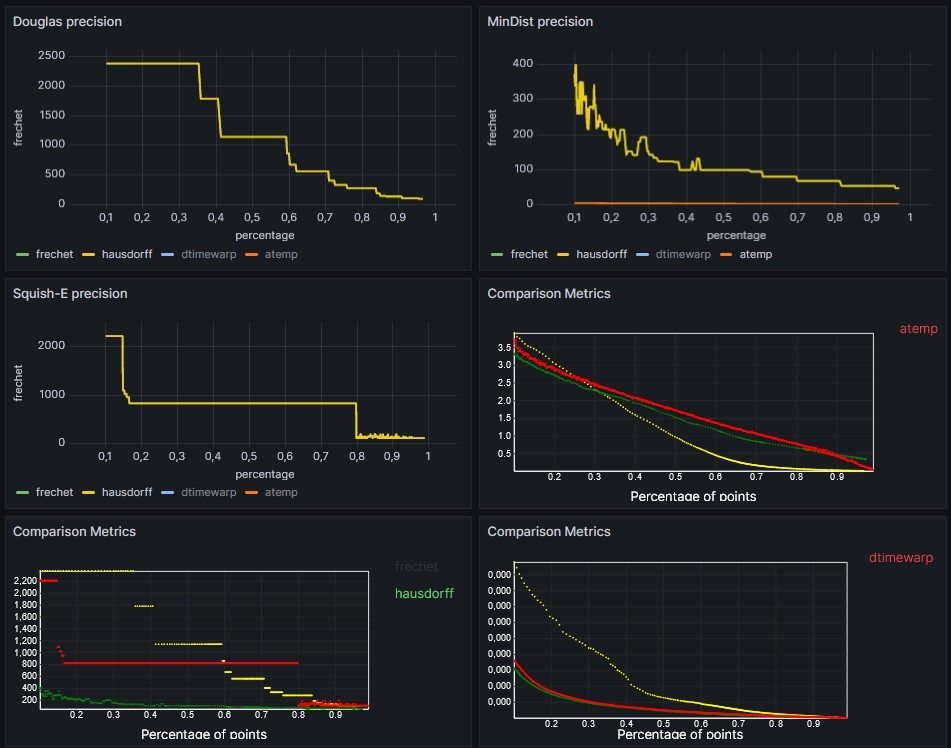
\includegraphics[width=1\linewidth]{figures/Stats/DashBoardright.jpg}
	\caption{Right panel of the Dashboard. }
	\label{fig:dashright}
\end{figure}

The graphs are interactive, allowing comparisons to be made. The Grafana plugin for the XY graph is useful but incomplete because the comparison graph is difficult to read. The dashboard contains highly useful information that can be retrieved to provide a more comprehensive perspective. Here are a few graphs that can be generated from dashboard data. Using a plot to read the extracted data :

\begin{figure}
	\centering
	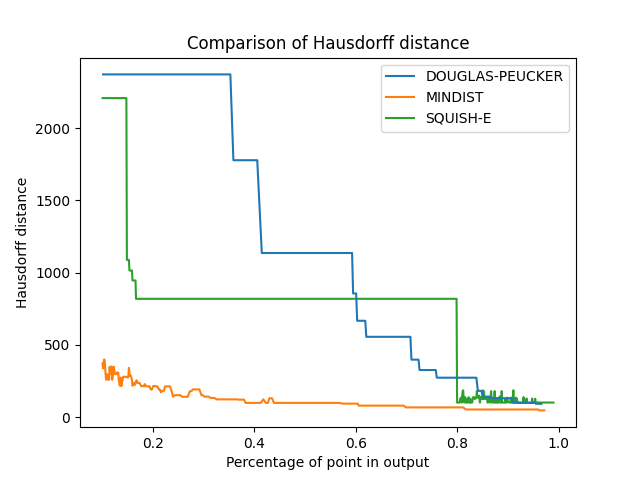
\includegraphics[width=0.9\linewidth]{figures/Stats/hausdorff_comp.png}
	\caption{Comparison of Hausdorff distance between MinDist, Douglas-Peucker, and SQUISH-E algorithms by percentage of points in output for Trajectory 1.}
	\label{fig:comp_h}
\end{figure}

The Hausdorff distance graphs in Figure \ref{fig:comp_h} indicate that the SQUISH-E algorithm often has greater values than Douglas-Peucker and MinDist across the whole range of percentages. Douglas-Peucker and MinDist retain shorter and more stable Hausdorff distances, indicating superior maximum deviation performance. SQUISH-E's lower competitive ratio shows that it performs better than Douglas-Peucker at keeping the original shape.

\begin{figure}
	\centering
	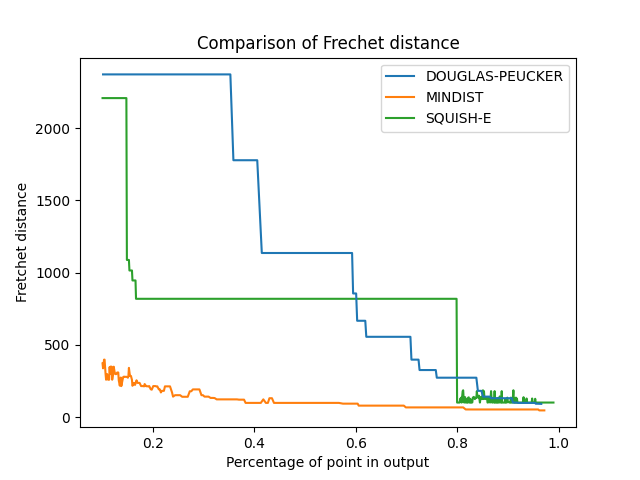
\includegraphics[width=0.9\linewidth]{figures/Stats/fretchet_comp.png}
	\caption{Comparison of Frechet distance between MinDist, Douglas-Peucker, and SQUISH-E algorithms by percentage of points in output for Trajectory 1.}
	\label{fig:comp_f}
\end{figure}

SQUISH-E has much larger Frechet distance values than MinDist, as seen in Figure \ref{fig:comp_f}. SQUISH-E performs similarly to Douglas-Peucker, particularly in the middle range. However, SQUISH-E's competitive ratio is almost always less than one. There is a similar finding for Hausdorff.



\begin{figure}
	\centering
	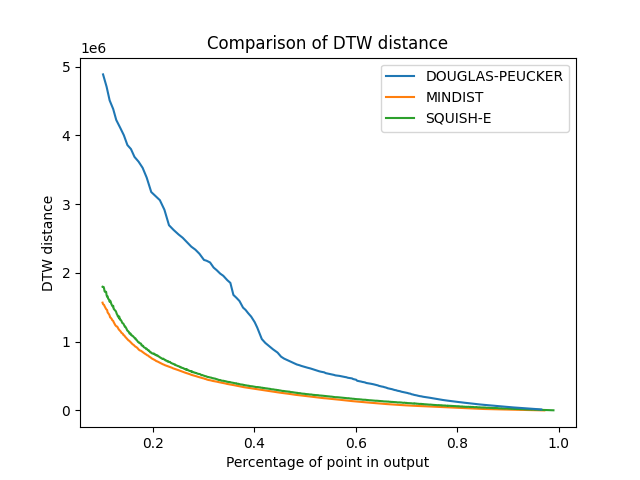
\includegraphics[width=0.9\linewidth]{figures/Stats/dtimewarp_comp.png}
	\caption{Comparison of DTW distance between MinDist, Douglas-Peucker, and SQUISH-E algorithms by percentage of points in output for Trajectory 1.}
	\label{fig:comp_dt}
\end{figure}

Figure \ref{fig:comp_dt} shows that SQUISH-E has lower DTW distances than Douglas-Peucker and MinDist. SQUISH-E is very near to MinDist and maintains a high accuracy level.  

\begin{figure}
	\centering
	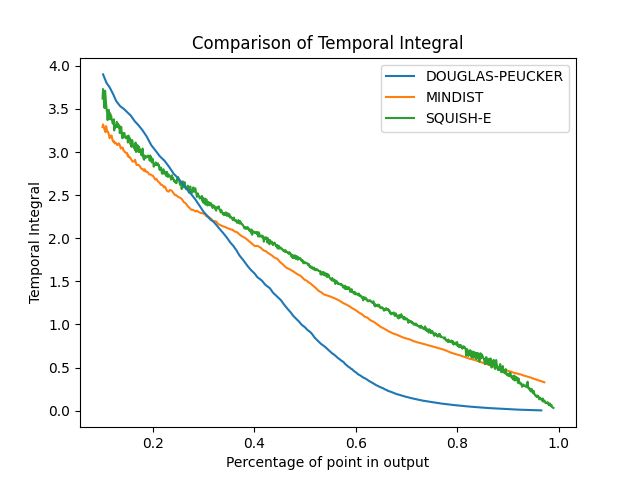
\includegraphics[width=0.9\linewidth]{figures/Stats/atemp_comp.png}
	\caption{Comparison of Temporal Integral between MinDist, Douglas-Peucker, and SQUISH-E algorithms by percentage of points in output for Trajectory 1.}
	\label{fig:comp_at}
\end{figure}

In Figure \ref{fig:comp_at}, SQUISH-E demonstrates superior performance in aggregate difference over the time period as evidenced by its consistently lower values when compared to Douglas-Peucker and MinDist for the Temporal Integral.
\\

The comparison of accuracies on trajectory 1 amongst the three algorithms (Douglas, SQUISH-E, and MindDist) is displayed in the following figures \labelcref{fig:comp_at,fig:comp_dt,fig:comp_f,fig:comp_h}. This is where the error distance variation with the compression level may be seen. For Douglas-Peucker and SQUISH-E, Frechet and Hausdorff's error level has a staircase structure, while for MinDist, it continuously lowers. With the exception of \ref{fig:comp_at}, where SQUISH-E performs worse but is still extremely close to its rivals, SQUISH-E is typically better than Douglas-Peucker and worse than MinDist.

\paragraph{Trajectory 2}

This trajectory in the Figure \ref{fig:traj2} is composed of 16310 points and begin at 1am the 8/1/2021 with a duration of 1 day. This trajectory is exceptional and allows us to observe specific cases such as round trips and breakpoints. This is useful for observing the behaviour of compression algorithms for this type of trajectory. 

\begin{figure}
	\centering
	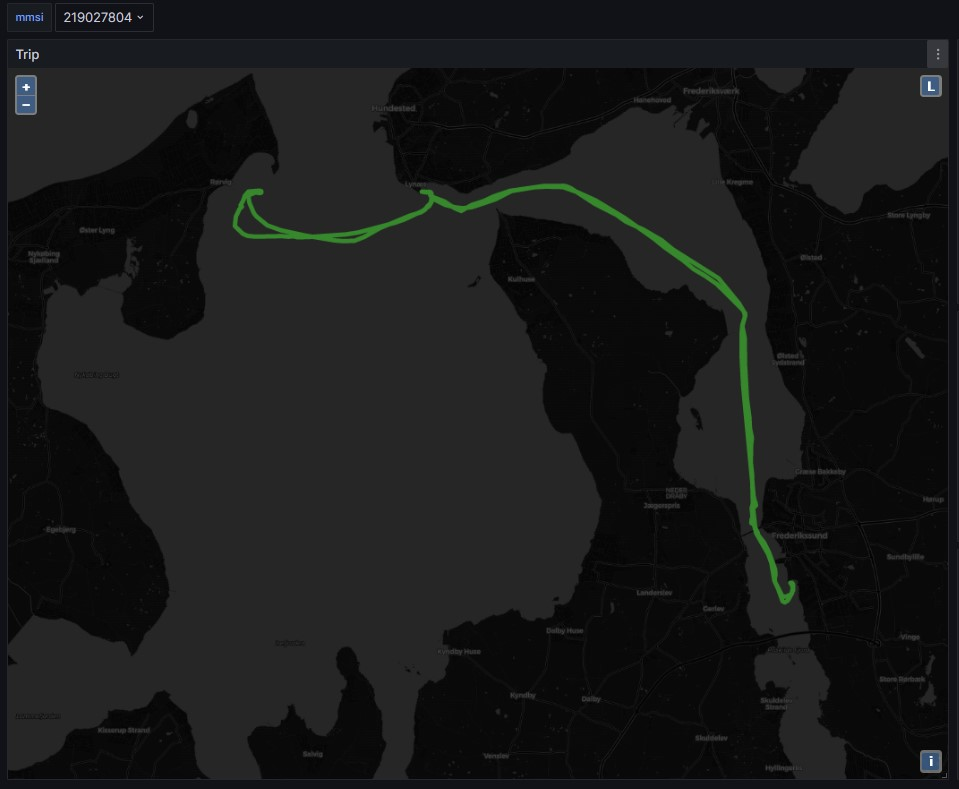
\includegraphics[width=0.7\linewidth]{figures/Stats/traj2.jpg}
	\caption{Trajectory 2 on a map.}
	\label{fig:traj2}
\end{figure}


\begin{figure}
	\centering
	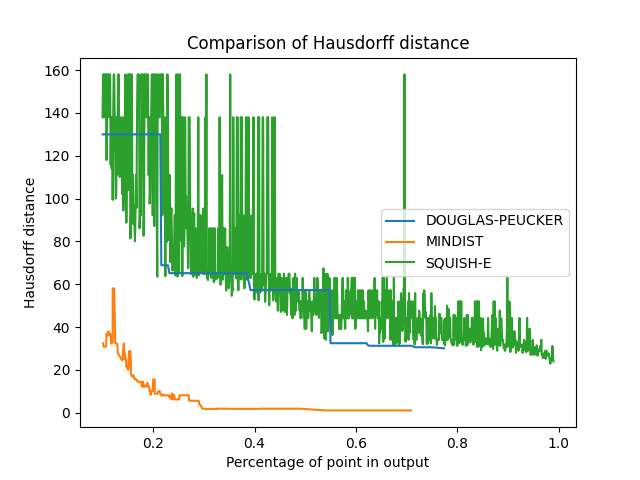
\includegraphics[width=0.9\linewidth]{figures/Stats/hausdorff_comp2.png}
	\caption{Comparison of Hausdorff distance between MinDist, Douglas-Peucker, and SQUISH-E algorithms by percentage of points in output  for Trajectory 2.}
	\label{fig:comp_h2}
\end{figure}

SQUISH-E typically has greater values than Douglas-Peucker and MinDist across the whole range of percentages, according to the Hausdorff distance graphs in Figure \ref{fig:comp_h2}. Douglas-Peucker and MinDist retain shorter and more stable Hausdorff distances, indicating superior maximum deviation performance. The competitive ratio for SQUISH-E is greater than one, indicating lower performance when compared to the other algorithms. \\

\begin{figure}
	\centering
	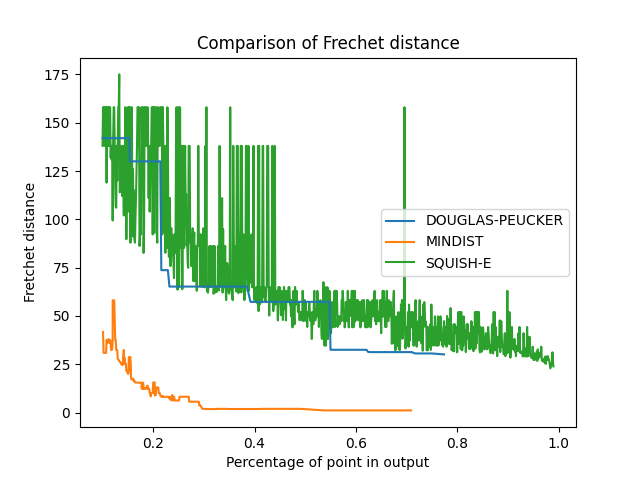
\includegraphics[width=0.9\linewidth]{figures/Stats/fretchet_comp2.png}
	\caption{Comparison of Frechet distance between MinDist, Douglas-Peucker, and SQUISH-E algorithms by percentage of points in output  for Trajectory 2.}
	\label{fig:comp_f2}
\end{figure}

In Figure \ref{fig:comp_f2}, SQUISH-E has substantially larger Frechet distance values than MinDist, yet there are many oscillations over the range. SQUISH-E performs similarly to Douglas-Peucker, particularly in the middle percentage range. However, the competitive ratio for SQUISH-E remains greater than one, indicating that it performs worse in retaining shape similarity than MinDist but is comparable to Douglas-Peucker in some ranges. \\

\begin{figure}
	\centering
	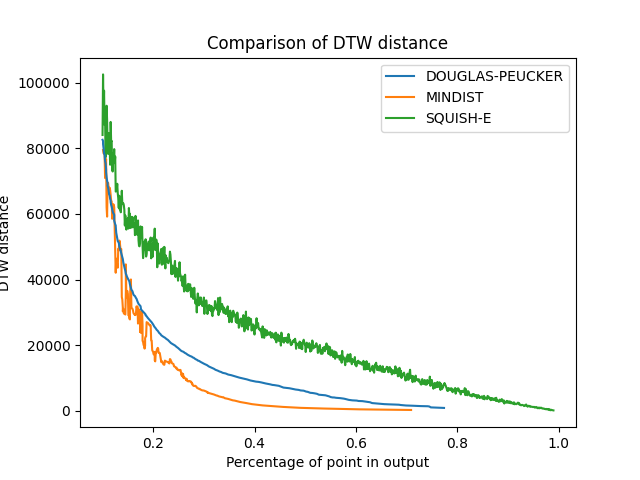
\includegraphics[width=0.9\linewidth]{figures/Stats/dtimewarp_comp2.png}
	\caption{Comparison of DTW distance between MinDist, Douglas-Peucker, and SQUISH-E algorithms by percentage of points in output  for Trajectory 2.}
	\label{fig:comp_dt2}
\end{figure}

Figure \ref{fig:comp_dt2} shows that SQUISH-E starts with higher DTW distances than Douglas-Peucker and MinDist. Around the 0.5 to 0.6 percentage point, SQUISH-E approaches Douglas-Peucker's performance but falls short of MinDist's reduced DTW distances. Initially, SQUISH-E has a higher competitive ratio, which improves over time but remains more than one, showing that it approaches Douglas-Peucker but not MinDist. \\

\begin{figure}
	\centering
	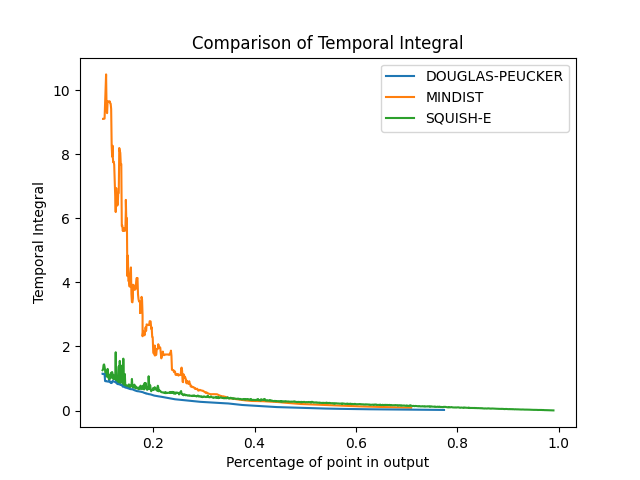
\includegraphics[width=0.9\linewidth]{figures/Stats/atemp_comp2.png}
	\caption{Comparison of Temporal Integral between MinDist, Douglas-Peucker, and SQUISH-E algorithms by percentage of points in output  for Trajectory 2.}
	\label{fig:comp_at2}
\end{figure}

In comparison to Douglas-Peucker and MinDist, SQUISH-E consistently displays lower values for the temporal integral area in Figure \ref{fig:comp_at2}, showing greater performance in aggregate difference over the time range. SQUISH-E is effective at preserving a lower cumulative deviation from the original data, as evidenced by its competitive ratio of less than 1.\\

SQUISH-E demonstrates strengths in specific metrics such as Temporal integral area, where it consistently outperforms Douglas-Peucker and MinDist. This is particularly notable given the dataset's characteristics, which include stop points and round-trip trajectories. However, SQUISH-E struggles with Frechet distance and Hausdorff distance, maintaining higher values (worse performance) across the range. The DTW distance metric shows some improvement for SQUISH-E, with the algorithm approaching the performance of Douglas-Peucker at higher percentages but not quite reaching the performance of MinDist. These insights highlight the areas where SQUISH-E excels and where it needs improvement relative to its competitors. MinDist has shown a really amazing result but the type of input make him difficult to use for use case as it is a distance. As we also saw because MinDist does not take into account temporality it has some issues on temporal metrics like in the figure \ref{fig:comp_at2}.

